\section{연구 결과}
 제작한 GS-system의 구동부 및 제어부는 스테핑 모터의 제어를 포함하는, 소형 천체망원경의 자동화를 위한 여러가지 편의기능들로 이루어져 있다. 하지만 회로도 상의 문제로, PC와 Firmware상의 연결을 담당하는 SerialPort를 제어하는 핀인 RX,TX핀(각각 0,1번 핀)을 모터를 제어하는 핀과 연결하였기 때문에 스테핑 모터의 제어는 성공하지 못하였다. 때문에 본 문단에서는 모터 제어를 제외한 소형 천체망원경의 자동화를 위한 여러가지 편의기능들의 제어를 어떤 방법으로 성공하였는지 서술한다.

\subsection{구동부 및 제어부}

\subsubsection{Firmware하드웨어}

	\begin{figure}[ht]
	\begin{center}
		\begin{tikzpicture}
		\node[anchor=south west,inner sep=0] at (0,0) 
		{
			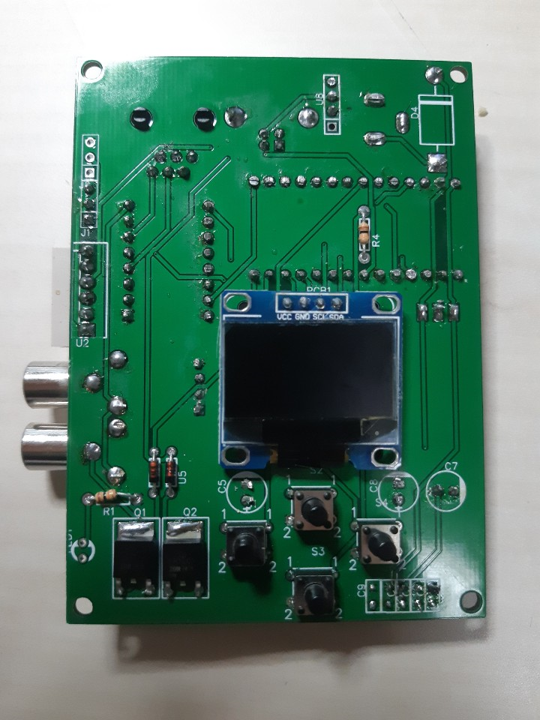
\includegraphics[height=6.5cm]{pcb1}
			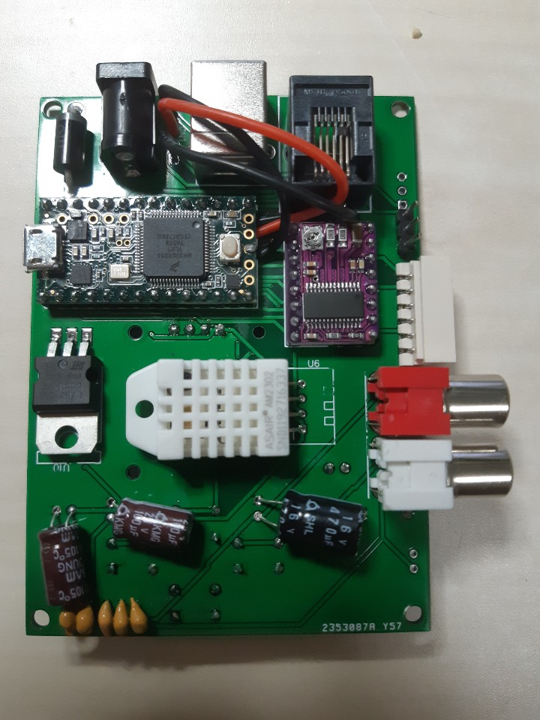
\includegraphics[height=6.5cm]{pcb2} 
		};
		\draw (0.35, 0.3) node {(a)};
		\draw (5.3, 0.3) node {(b)};
		\end{tikzpicture}
	\end{center}
	\caption{완성된 Firmware하드웨어의 (a)앞면 과 (b)뒷면}
	\label{pcb}
	\end{figure}
	
완성한 Firmware하드웨어의 PCB 는\textrm{Figure}. \ref{pcb}과 같다. PCB의 앞면에는 오프라인 제어를 편리하게 하기 위한, 메뉴시스템을 활용할 수 있도록 $128 \times 64 OLED$를 활용하였으며, 이를 제어할 수 있도록 버튼 4개를 같이 사용하였다. PCB의 뒷면에는 전원의 공급 및 여러 편의기능들을 위한 연결단자들을 배치하였다.
 
	
	
\subsubsection{하드웨어의 Menu조작}
 
  \begin{figure}[h]
 	\begin{center}
 		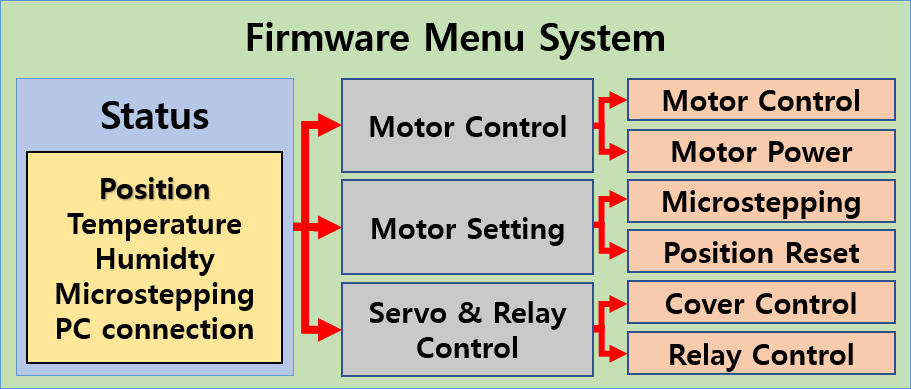
\includegraphics[width = 11cm]{menu}
 	\end{center}
 	\caption{제작한 Firmware하드웨어의 Menu System의 구성}
 	\label{menu}
 \end{figure}
 

연구과정에서 소개하였듯, 하드웨어의 Menu 조작으로 대부분의 편의기능들이 이용하능하다. 이용이 가능한 편의기능들은 Position Reset, Microstepping 설정, 덮개 개폐, 릴레이 스위치 제어 등이 있다. \textrm{Figure}. \ref{menu}는 사용가능한 함수 및 Menu System의 구성에 대하여 정리한 표이며, \textrm{Figure}. \ref{mask_status}는 실제로 제작한 Firmware하드웨어의 메뉴 시스템을 통한 망원경 덮개의 개폐를 제어하는 모습이다. 화면 아래의 버튼들을 이용해 덮개를 제어할 수 있으며, 제어 상태를 확인할 수 있다.

	\begin{figure}[ht]
	\begin{center}
		\begin{tikzpicture}
		\node[anchor=south west,inner sep=0] at (0,0) 
		{
			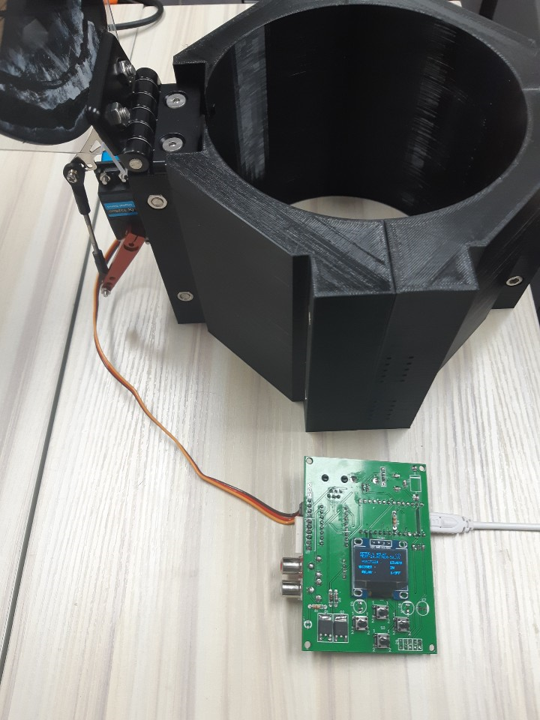
\includegraphics[height=6.5cm]{mask_status1}
			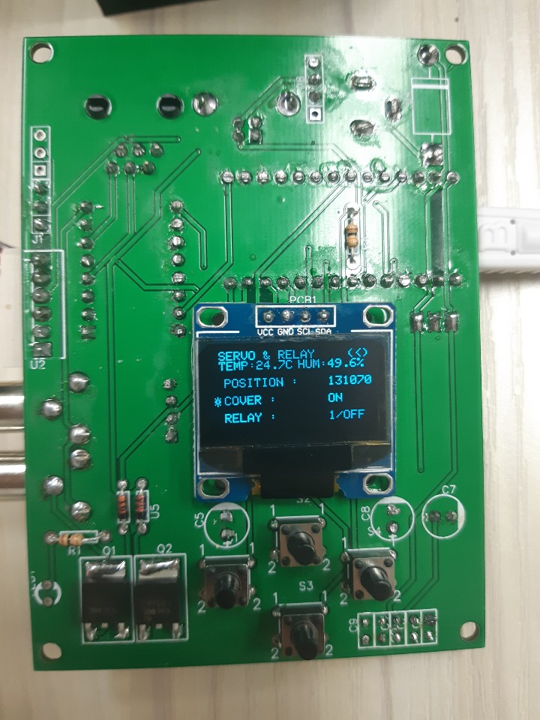
\includegraphics[height=6.5cm]{mask_status2} 
		};
		\draw (0.35, 0.3) node {(a)};
		\draw (5.3, 0.3) node {(b)};
		\end{tikzpicture}
	\end{center}
	\caption{(a) 개선된 모터포커서를 이용하여 제어한 덮개 (b) 이 때 개선된 모터 포커서에 출력되는 마스크의 상태}
	\label{mask_status}
\end{figure}
 
\newpage

\subsection{제어부 (ASCOM Driver)}


 기존의 모터포커서의 여러 기능들이 추가됨에 따라, 기존에 만들었던 ASCOM 호환 드라이버 또한 업데이트를 할 필요성이 있었다. 때문에 여러가지 기능들을 추가하여 기존의 GUI를 발전시켰으며, \textrm{Figure}.\ref{maincontrol}은 발전시킨 ASCOM 드라이버의 GUI의 모습을 나타내었다.
 
 \begin{figure}[h]
	\begin{center}
		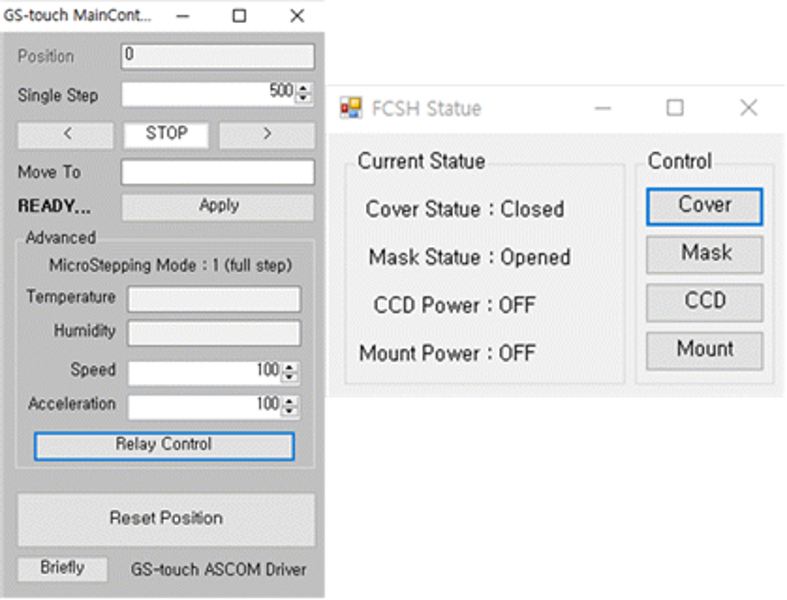
\includegraphics[width = 11cm]{maincontrol}
	\end{center}
	\caption{개선된 제어부의 GUI 모습}
	\label{maincontrol}
\end{figure}

 기존의 GS-touch에서 추가된 기능인 덮개 제어기능, 열선 제어기능, 릴레이 스위치의 제어기능을 포함하고 있으며, 각각의 릴레이 스위치가 제어하는 기능들을 적었다.
